\documentclass{article}
\usepackage{civ}
\newcommand*{\tabbox}[2][t]{%
    \vspace{0pt}\parbox[#1][3.7\baselineskip]{1cm}{\strut#2\strut}}
\title{CIV102: Problem Set \#8}
\author{QiLin Xue \\ \href{mailto:qilin.xue@mail.utoronto.ca}{qilin.xue@mail.utoronto.ca} \\ TA: Michel}
\everymath{\displaystyle}
\usepackage{multirow}
\date{\today}
\usepackage{mathrsfs}
\usetikzlibrary{arrows}
\usetikzlibrary{arrows.meta}
\usepackage{siunitx}
\usepackage{wasysym}
\usetikzlibrary{calc}
\usepackage{xcolor}
\setlength\parindent{0pt}
% \setlength\extrarowheight{10pt}
\renewcommand{\arraystretch}{2}
\usepackage{adjustbox}
\begin{document}
\maketitle
\section{Problem One}
\textbf{(a)} We first perform the analysis for the beam on the left. Let the two reaction forces be $A$ and $C$. Note that there are no horizontal forces from $A$ since the net horizontal force is zero. Then:
\begin{equation}
    A + C = P
\end{equation}
and balancing torques:
\begin{equation}
    P\left(\frac{3L}{4}\right) = C\left(L\right) \implies C = \frac{3}{4}P
\end{equation}
and similarly $A=\frac{1}{4}P$. The shear force diagram can be drawn as:
\begin{center}
    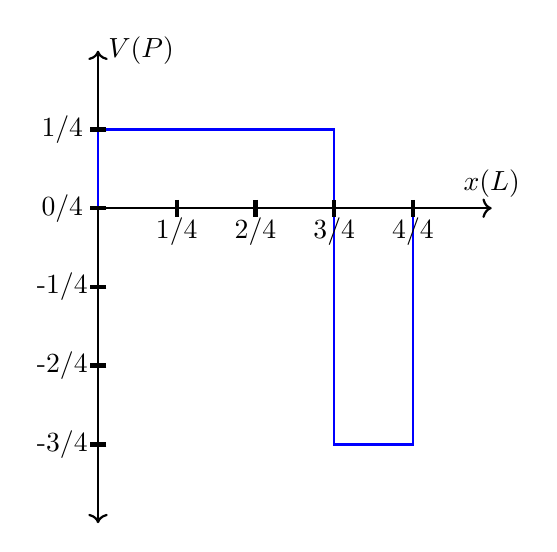
\begin{tikzpicture}

        % Axis
        \draw[thick,->] (0,0) -- (5,0) node[above] {$x(L)$};
        \draw[thick,<->] (0,-4) -- (0,2) node[right] {$V(P)$};

        % Actual Plot
        \draw[thick, blue] (0,0) -- (0,1) -- (3,1) -- (3,-3) -- (4,-3) -- (4,0);

        % X axis
        \foreach \x in {1,2,...,4}
        {        
          \coordinate (A\x) at ($(0,0)+(\x,0)$) {};
          \draw[ultra thick] ($(A\x)+(0,3pt)$) -- ($(A\x)-(0,3pt)$);
          \node at ($(A\x)+(0ex,-2ex)$) {\x/4};
        }

        % Y Axis
        \foreach \y in {-3,-2,...,1}
        {        
          \coordinate (B\y) at ($(0,0)+(0,\y)$) {};
          \draw[ultra thick] ($(B\y)+(3pt,0)$) -- ($(B\y)-(3pt,0)$);
          \node at ($(B\y)+(-3ex,0)$) {\y/4};
        }
    \end{tikzpicture}
\end{center}
and the moment diagram:
\begin{center}
    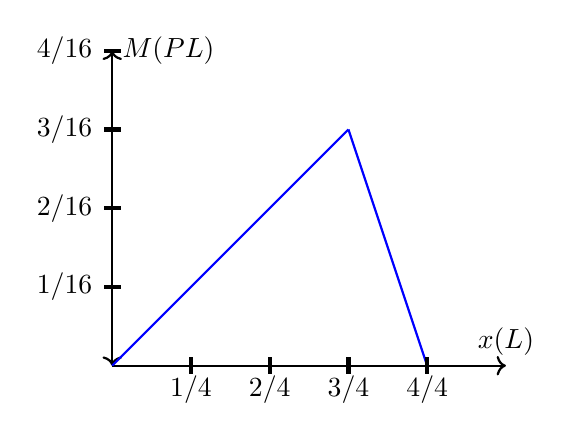
\begin{tikzpicture}

        % Axis
        \draw[thick,->] (0,0) -- (5,0) node[above] {$x(L)$};
        \draw[thick,<->] (0,0) -- (0,4) node[right] {$M(PL)$};

        % Actual Plot
        \draw[thick, blue] (0,0) -- (3,3);
        \draw[thick, blue] (4,0) -- (3,3);

        % X axis
        \foreach \x in {1,2,...,4}
        {        
          \coordinate (A\x) at ($(0,0)+(\x,0)$) {};
          \draw[ultra thick] ($(A\x)+(0,3pt)$) -- ($(A\x)-(0,3pt)$);
          \node at ($(A\x)+(0ex,-2ex)$) {\x/4};
        }

        % Y Axis
        \foreach \y in {1,2,...,4}
        {        
          \coordinate (B\y) at ($(0,0)+(0,\y)$) {};
          \draw[ultra thick] ($(B\y)+(3pt,0)$) -- ($(B\y)-(3pt,0)$);
          \node at ($(B\y)+(-4ex,0)$) {\y/16};
        }
    \end{tikzpicture}
\end{center}
and the curvature diagram:
\begin{center}
    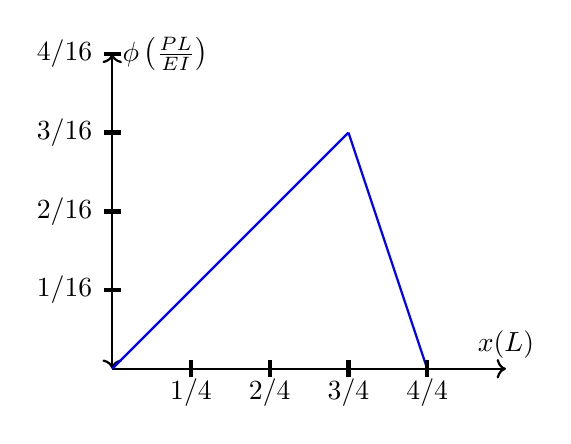
\begin{tikzpicture}

        % Axis
        \draw[thick,->] (0,0) -- (5,0) node[above] {$x(L)$};
        \draw[thick,<->] (0,0) -- (0,4) node[right] {$\phi\left(\frac{PL}{EI}\right)$};

        % Actual Plot
        \draw[thick, blue] (0,0) -- (3,3);
        \draw[thick, blue] (4,0) -- (3,3);

        % X axis
        \foreach \x in {1,2,...,4}
        {        
          \coordinate (A\x) at ($(0,0)+(\x,0)$) {};
          \draw[ultra thick] ($(A\x)+(0,3pt)$) -- ($(A\x)-(0,3pt)$);
          \node at ($(A\x)+(0ex,-2ex)$) {\x/4};
        }

        % Y Axis
        \foreach \y in {1,2,...,4}
        {        
          \coordinate (B\y) at ($(0,0)+(0,\y)$) {};
          \draw[ultra thick] ($(B\y)+(3pt,0)$) -- ($(B\y)-(3pt,0)$);
          \node at ($(B\y)+(-4ex,0)$) {\y/16};
        }
    \end{tikzpicture}
\end{center}
The deflection at $B$ with respect to the tangent line at $A$ is:
\begin{equation}
    \delta_{BA} = \bar{x}_{BA}\int_B^A \phi(x) \dd{x} = \left(\frac{1}{3}\frac{3L}{4}\right)\left(\frac{1}{2}\frac{3L}{4}\frac{3}{16}\frac{PL}{EI}\right) = \frac{9}{512}\frac{PL^3}{EI}
    \label{eq:}
\end{equation}
The deflection at $C$ with respect to the tangent line at $A$ is:
\begin{equation}
    \delta_{CA} = \left(\frac{2}{3}\frac{L}{4}\right)\left(\frac{1}{2}\frac{L}{4}\frac{3}{16}\frac{PL}{EI}\right)+\left(\frac{L}{4}+\frac{1}{3}\frac{3L}{4}\right)\left(\frac{1}{2}\frac{3L}{4}\frac{3}{16}\frac{PL}{EI}\right)=\left(\frac{1}{256}+\frac{9}{256}\right)\frac{PL^3}{EI}=\frac{5}{128}\frac{PL^3}{EI}
    \label{eq:}
\end{equation}

The angle the beam makes at $A$ is given by:
\begin{equation}
    \theta_A \cong \frac{5}{128}\frac{PL^2}{EI}
    \label{eq:}
\end{equation}
so the deflection of $B$ with respect to the initial position is:
\begin{equation}
    \Delta_B = \frac{3}{4}L\theta_A-\delta_{BA} = \frac{15}{512}\frac{PL^3}{EI}-\frac{9}{512}\frac{PL^3}{EI}=\frac{3}{256}\frac{PL^3}{EI} 
    \label{eq:}
\end{equation}
\textbf{(b)} Again, since there are no net horizontal forces, the reaction force at the left end is completely vertical, which we denote as $A$ which is equal and opposite to $P$. It also exerts a counterclockwise moment with a magnitude equal to $M_A=PL$. Therefore, the shear force and moment diagrams are:
\begin{center}
    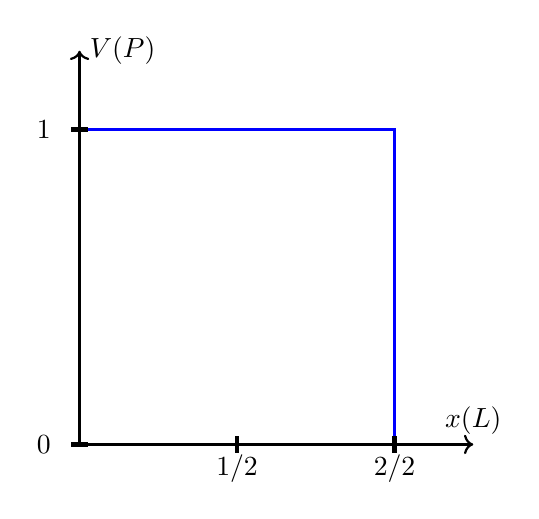
\begin{tikzpicture}

        % Axis
        \draw[thick,->] (0,0) -- (5,0) node[above] {$x(L)$};
        \draw[thick,->] (0,0) -- (0,5) node[right] {$V(P)$};

        % Actual Plot
        \draw[thick, blue] (0,4) -- (4,4) -- (4,0);

        % X axis
        \foreach \x in {1,2}
        {        
          \coordinate (A\x) at ($(0,0)+(2*\x,0)$) {};
          \draw[ultra thick] ($(A\x)+(0,3pt)$) -- ($(A\x)-(0,3pt)$);
          \node at ($(A\x)+(0ex,-2ex)$) {\x/2};
        }

        % Y Axis
        \foreach \y in {0,1}
        {        
          \coordinate (B\y) at ($(0,0)+(0,4*\y)$) {};
          \draw[ultra thick] ($(B\y)+(3pt,0)$) -- ($(B\y)-(3pt,0)$);
          \node at ($(B\y)+(-3ex,0)$) {\y};
        }
    \end{tikzpicture}
\end{center}
and the moment diagram:
\begin{center}
    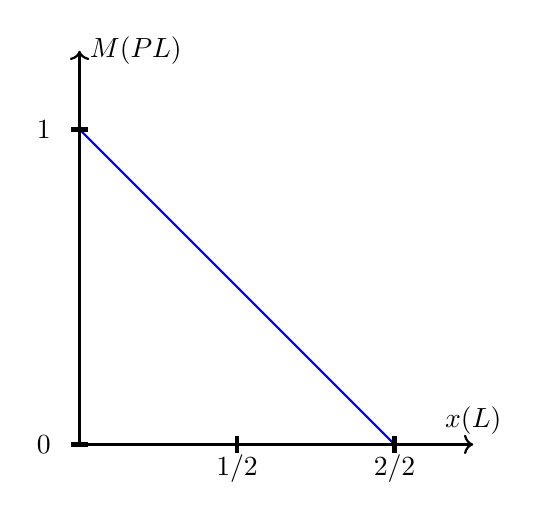
\begin{tikzpicture}

        % Axis
        \draw[thick,->] (0,0) -- (5,0) node[above] {$x(L)$};
        \draw[thick,->] (0,0) -- (0,5) node[right] {$M(PL)$};

        % Actual Plot
        \draw[thick, blue] (0,4) -- (4,0);

        % X axis
        \foreach \x in {1,2}
        {        
          \coordinate (A\x) at ($(0,0)+(2*\x,0)$) {};
          \draw[ultra thick] ($(A\x)+(0,3pt)$) -- ($(A\x)-(0,3pt)$);
          \node at ($(A\x)+(0ex,-2ex)$) {\x/2};
        }

        % Y Axis
        \foreach \y in {0,1}
        {        
          \coordinate (B\y) at ($(0,0)+(0,4*\y)$) {};
          \draw[ultra thick] ($(B\y)+(3pt,0)$) -- ($(B\y)-(3pt,0)$);
          \node at ($(B\y)+(-3ex,0)$) {\y};
        }
    \end{tikzpicture}
\end{center}
For the curvature diagram, we have:
\begin{center}
    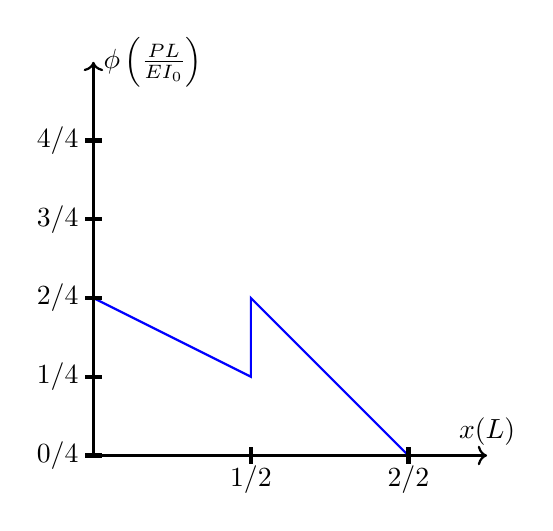
\begin{tikzpicture}

        % Axis
        \draw[thick,->] (0,0) -- (5,0) node[above] {$x(L)$};
        \draw[thick,->] (0,0) -- (0,5) node[right] {$\phi\left(\frac{PL}{EI_0}\right)$};

        % Actual Plot
        \draw[thick, blue] (0,2) -- (2,1) -- (2,2) -- (4,0);

        % X axis
        \foreach \x in {1,2}
        {        
          \coordinate (A\x) at ($(0,0)+(2*\x,0)$) {};
          \draw[ultra thick] ($(A\x)+(0,3pt)$) -- ($(A\x)-(0,3pt)$);
          \node at ($(A\x)+(0ex,-2ex)$) {\x/2};
        }

        % Y Axis
        \foreach \y in {0,1,2,3,4}
        {        
          \coordinate (B\y) at ($(0,0)+(0,\y)$) {};
          \draw[ultra thick] ($(B\y)+(3pt,0)$) -- ($(B\y)-(3pt,0)$);
          \node at ($(B\y)+(-3ex,0)$) {\y/4};
        }
    \end{tikzpicture}
\end{center}
where the varying moment of inertia was taken into consideration. The deflection of point $C$ is then given as:
\begin{equation}
    \delta_{CA} = \bar{x}_1A_\text{right triangle} + \bar{x}_2A_\text{rectangle} + \bar{x}A_\text{top left triangle}
    \label{eq:}
\end{equation}
where we have broken up the curvature diagram into three shapes by breaking the trapezoidal shape into a rectangle and a triangle. Thus:
\begin{align}
    \delta_{CA}&=\left(\frac{2}{3}\frac{L}{2}\right)\left(\frac{1}{2}\frac{L}{2}\frac{1}{2}\frac{PL}{EI_0}\right)+\left(\frac{L}{2}+\frac{1}{2}\frac{L}{2}\right)\left(\frac{L}{2}\frac{1}{4}\frac{PL}{EI_0}\right)+\left(\frac{L}{2}+\frac{2}{3}\frac{L}{2}\right)\left(\frac{1}{2}\frac{L}{2}\frac{1}{4}\frac{PL}{EI_0}\right) \\ &= \left(\frac{1}{24}+\frac{3}{32}+\frac{5}{96}\right)\frac{PL^3}{EI_0} \\ &=\frac{3}{16}\frac{PL^3}{EI_0}
\end{align}
Since $A$ is a horizontal tangent, the displacement of point $C$ is:
\begin{equation}
    \Delta_C = \frac{3}{16}\frac{PL^3}{EI_0}
    \label{eq:}
\end{equation}

\newpage
\section{Problem Two}
We can find the force $F$ exerted by the supports due to symmetry. We have:
\begin{equation}
  25(7) = 2F \implies F = 87.5\si{\kilo\newton}
  \label{eq:}
\end{equation}
The shear force diagram looks like:
\begin{center}
  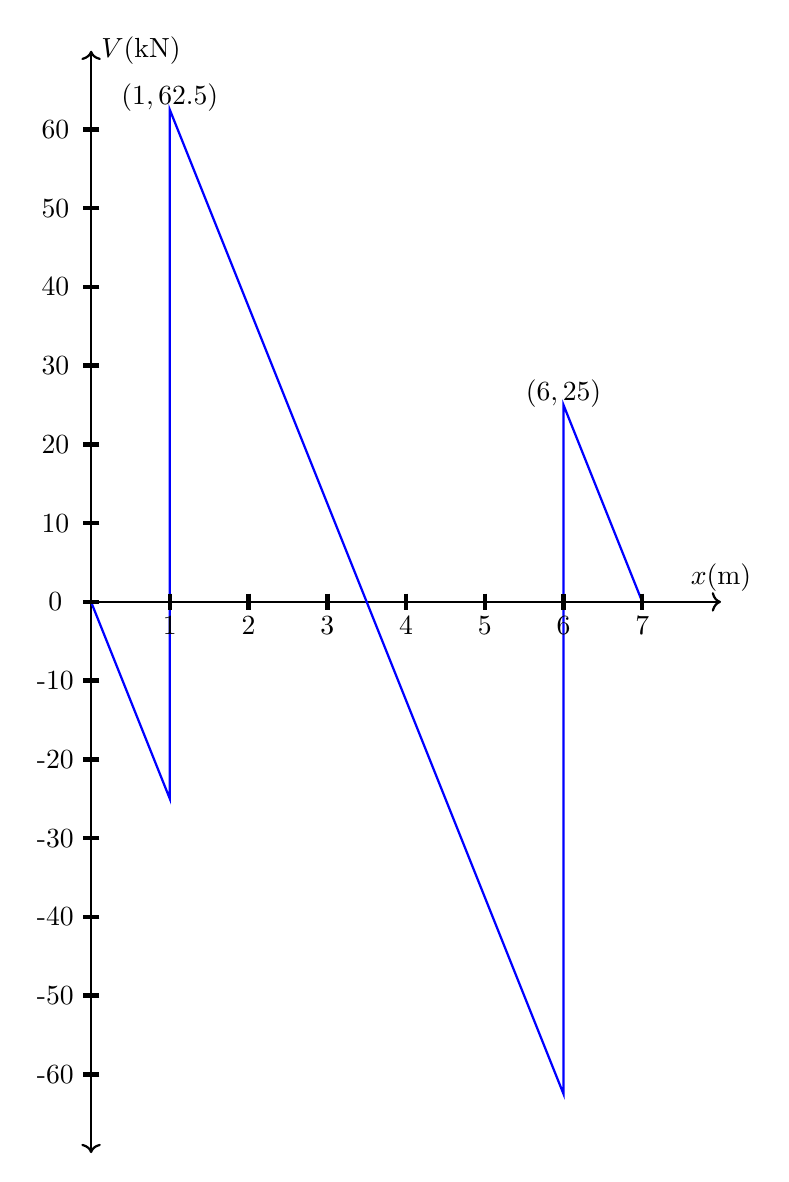
\begin{tikzpicture}

      % Axis
      \draw[thick,->] (0,0) -- (8,0) node[above] {$x(\si{\meter})$};
      \draw[thick,<->] (0,-7) -- (0,7) node[right] {$V(\si{\kilo\newton})$};

      % Actual Plot
      \draw[thick, blue] (0,0) -- (1,-2.5) -- (1,6.25) -- (6,-6.25) -- (6, 2.5) -- (7, 0);

      % X axis
      \foreach \x in {1,2,3,4,5,6,7}
      {        
        \coordinate (A\x) at ($(0,0)+(\x,0)$) {};
        \draw[ultra thick] ($(A\x)+(0,3pt)$) -- ($(A\x)-(0,3pt)$);
        \node at ($(A\x)+(0ex,-2ex)$) {\x};
      }

      % Y Axis
      \foreach \y in {-60,-50,...,60}
      {        
        \coordinate (B\y) at ($(0,0)+(0,\y/10)$) {};
        \draw[ultra thick] ($(B\y)+(3pt,0)$) -- ($(B\y)-(3pt,0)$);
        \node at ($(B\y)+(-3ex,0)$) {\y};
      }
      \node at ($(1,6.25)+(0,+1ex)$) {$(1,62.5)$};
      \node at ($(6,2.5)+(0,+1ex)$) {$(6,25)$};
  \end{tikzpicture}
\end{center}
The moment diagram looks like:
\begin{center}
  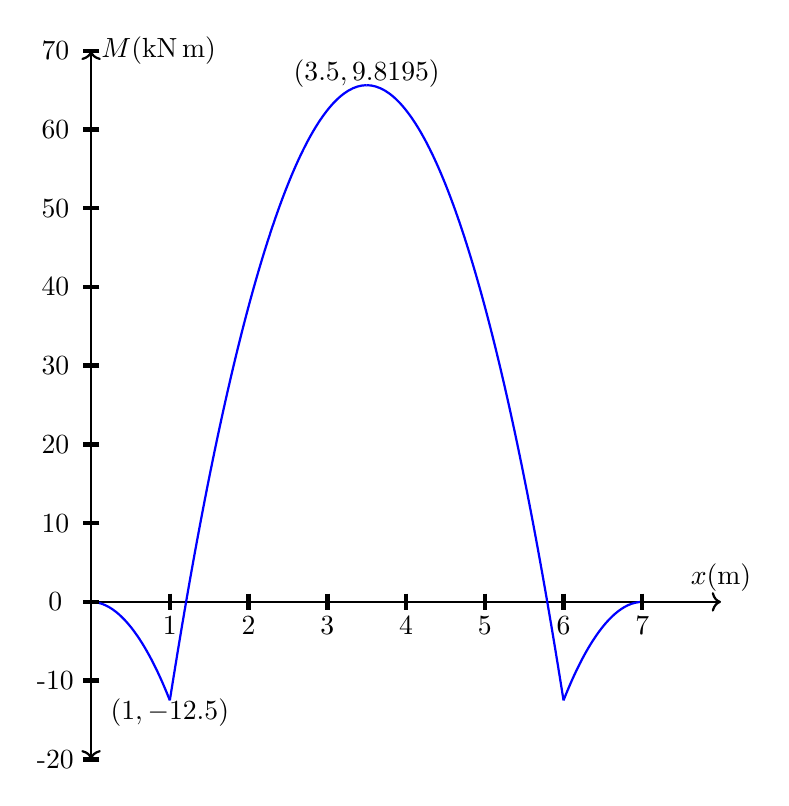
\begin{tikzpicture}

      % Axis
      \draw[thick,->] (0,0) -- (8,0) node[above] {$x(\si{\meter})$};
      \draw[thick,<->] (0,-2) -- (0,7) node[right] {$M(\si{\kilo\newton\meter})$};

      % Actual Plot
      \draw[thick, blue] (0,0) parabola (1,-1.25);
      \draw[thick, blue] (3.5,6.5625) parabola (1,-1.25);
      \draw[thick, blue] (3.5,6.5625) parabola (6,-1.25);
      \draw[thick, blue] (7,0) parabola (6,-1.25);


      -- (1,-2.5) -- (1,6.25) -- (6,-6.25) -- (6, 2.5) -- (7, 0);

      % X axis
      \foreach \x in {1,2,3,4,5,6,7}
      {        
        \coordinate (A\x) at ($(0,0)+(\x,0)$) {};
        \draw[ultra thick] ($(A\x)+(0,3pt)$) -- ($(A\x)-(0,3pt)$);
        \node at ($(A\x)+(0ex,-2ex)$) {\x};
      }

      % Y Axis
      \foreach \y in {-20,-10,...,70}
      {        
        \coordinate (B\y) at ($(0,0)+(0,\y/10)$) {};
        \draw[ultra thick] ($(B\y)+(3pt,0)$) -- ($(B\y)-(3pt,0)$);
        \node at ($(B\y)+(-3ex,0)$) {\y};
      }
      \node at ($(3.5,6.5625)+(0,+1ex)$) {$(3.5,9.8195)$};
      \node at ($(1,-1.25)+(0,-1ex)$) {$(1,-12.5)$};

  \end{tikzpicture}
\end{center}
Note that the intercepts are at $(1.209,0)$ and $(5.791,0)$, which represent locations where the moment is zero. The center of mass of the beam is:
\begin{equation}
  \bar{y} = \frac{\left(150\right)\left(125 \cdot 300\right)+\left(350\right)\left(800\cdot 100\right)}{800\cdot 100 + 125 \cdot 300} = 286.17 \si{\milli\meter}
  \label{eq:}
\end{equation}
from the bottom. The moment of inertia is then:
\begin{equation}
  I = \frac{1}{12}\left(800\right)\left(100\right)^3 + \left(800\cdot 100\right)\left(350-286.17\right)^2 + \frac{1}{12}\left(125\right)\left(300\right)^3 + \left(125\cdot 300\right)\left(286.17-150\right)^2 = 1369.19 \times 10^6 \si{\milli\meter\tothe{4}}
  \label{eq:}
\end{equation}
Therefore, the flexural stiffness is:
\begin{equation}
  EI = 4.1076 \times 10^{4} \si{\kilo\pascal\meter\squared} 
  \label{eq:}
\end{equation}
and the curvature diagram is simply scaled by the inverse of this:
\begin{center}
  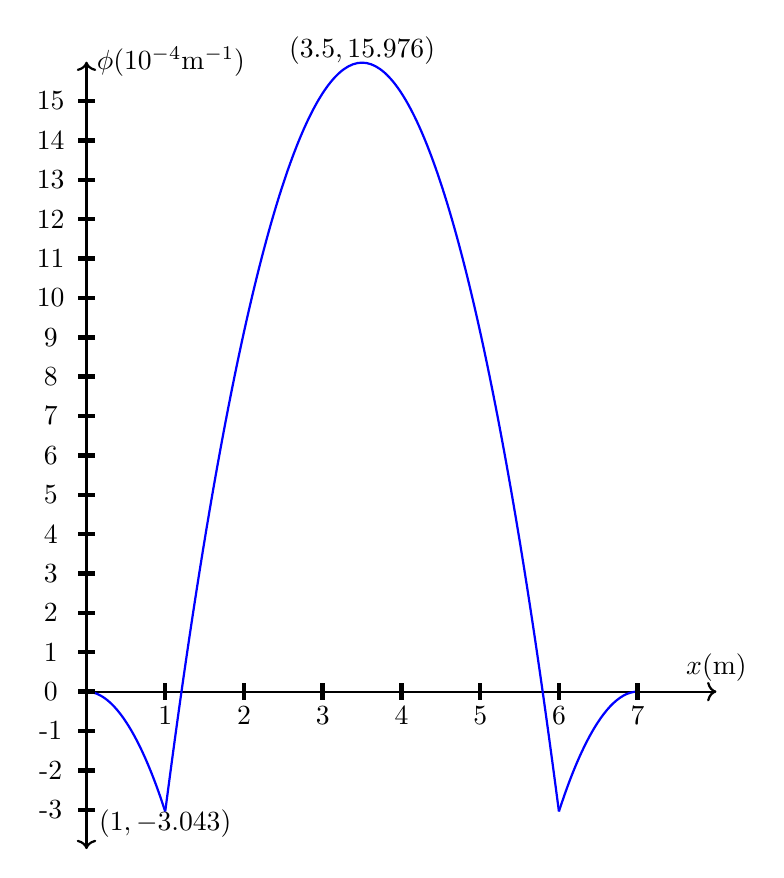
\begin{tikzpicture}

      % Axis
      \draw[thick,->] (0,0) -- (8,0) node[above] {$x(\si{\meter})$};
      \draw[thick,<->] (0,-2) -- (0,8) node[right] {$\phi (10^{-4}\si{\per\meter})$};

      % Actual Plot
      \draw[thick, blue] (0,0) parabola (1,-1.522);
      \draw[thick, blue] (3.5,7.988) parabola (1,-1.522);
      \draw[thick, blue] (3.5,7.988) parabola (6,-1.522);
      \draw[thick, blue] (7,0) parabola (6,-1.522);

      % X axis
      \foreach \x in {1,2,3,4,5,6,7}
      {        
        \coordinate (A\x) at ($(0,0)+(\x,0)$) {};
        \draw[ultra thick] ($(A\x)+(0,3pt)$) -- ($(A\x)-(0,3pt)$);
        \node at ($(A\x)+(0ex,-2ex)$) {\x};
      }

      % Y Axis
      \foreach \y in {-3,-2,-1,...,15}
      {        
        \coordinate (B\y) at ($(0,0)+(0,0.5*\y)$) {};
        \draw[ultra thick] ($(B\y)+(3pt,0)$) -- ($(B\y)-(3pt,0)$);
        \node at ($(B\y)+(-3ex,0)$) {\y};
      }
      \node at ($(3.5,7.988)+(0,+1ex)$) {$(3.5,15.976)$};
      \node at ($(1,-1.522)+(0,-1ex)$) {$(1,-3.043)$};

  \end{tikzpicture}
\end{center}
We can determine the equation of the curve in the middle to be:
\begin{equation}
  \phi(x) = -3.043\cdot10^{-4}\left(x-3.5\right)^{2}+15.976\cdot10^{-4}
\end{equation}
We can calculate the deflection at point $C$ to be:
\begin{align}
  \delta_{C,mid} &= \int_{C}^\text{mid} = \int_{3.5}^6 (6-x)\left(-3.043\cdot10^{-4}\left(x-3.5\right)^{2}+15.976\cdot10^{-4}\right) \dd{x} = 4.002\si{\milli\meter}
  \label{eq:}
\end{align}
Since the slope at the midpoint is zero, we don't have to do anything else. The beam looks like this:
\begin{center}
  \includegraphics[width=0.6\linewidth]{bad.png}
\end{center}
\newpage
\section{Problem Three}
\textbf{(a)} If we ignore $P_B$, then the forces exerted by the two supports $A$ and $C$ as $200\si{\kilo\newton}$ each, making the shear force diagram:
\begin{center}
  \begin{tikzpicture}[x=0.3cm,y=1cm]
      % Axis
      \draw[thick,->] (0,0) -- (28,0) node[above] {$x(\si{\meter})$};
      \draw[thick,->] (0,-3) -- (0,3) node[right] {$V(\si{\kilo\newton})$};

      % Actual Plot
      \draw[thick, blue] (0,0) -- (0,2) -- (7,2) -- (7,0) -- (21,0) -- (21,-2) -- (28,-2) -- (28,0);

      % X axis
      \foreach \x in {7,14,21,28}
      {        
        \coordinate (A\x) at ($(0,0)+(\x,0)$) {};
        \draw[ultra thick] ($(A\x)+(0,3pt)$) -- ($(A\x)-(0,3pt)$);
        \node at ($(A\x)+(0ex,-2ex)$) {\x};
      }

      % Y Axis
      \foreach \y in {-200,-100,...,200}
      {        
        \coordinate (B\y) at ($(0,0)+(0,\y/100)$) {};
        \draw[ultra thick] ($(B\y)+(3pt,0)$) -- ($(B\y)-(3pt,0)$);
        \node at ($(B\y)+(-3ex,0)$) {\y};
      }
  \end{tikzpicture}
\end{center}
and the moment diagram:
\begin{center}
  \begin{tikzpicture}[x=0.3cm,y=0.3cm]
      % Axis
      \draw[thick,->] (0,0) -- (30,0) node[above] {$x(\si{\meter})$};
      \draw[thick,->] (0,-3) -- (0,20) node[right] {$M(\si{\kilo\newton\meter})$};

      % Actual Plot
      \draw[thick, blue] (0,0) -- (7,14) -- (21,14) -- (28,0);

      % X axis
      \foreach \x in {7,14,21,28}
      {        
        \coordinate (A\x) at ($(0,0)+(\x,0)$) {};
        \draw[ultra thick] ($(A\x)+(0,3pt)$) -- ($(A\x)-(0,3pt)$);
        \node at ($(A\x)+(0ex,-2ex)$) {\x};
      }

      % Y Axis
      \foreach \y in {0,700,1400}
      {        
        \coordinate (B\y) at ($(0,0)+(0,\y/100)$) {};
        \draw[ultra thick] ($(B\y)+(3pt,0)$) -- ($(B\y)-(3pt,0)$);
        \node at ($(B\y)+(-3ex,0)$) {\y};
      }
  \end{tikzpicture}
\end{center}
We can abuse symmetry here to determine the displacement of point $C$ relative to $B$ as:
\begin{equation}
  \delta_{CB} = \Delta_{B} = \frac{1}{EI}\left(\frac{2}{3}(7)\right)\left(\frac{1}{2}(7)(1400)\right)+\left(7+\frac{7}{2}\right)\left(7\cdot 1400\right) = 628.(83)\si{\milli\meter}
  \label{eq:}
\end{equation}
which is true since the horizontal tangent at the midpoint is zero.

\textbf{(b)} Due to symmetry, the two supports would each exert a force of $P_B/2$. Therefore, the shear force diagram looks like
\begin{center}
  \begin{tikzpicture}[x=0.3cm,y=1cm]
      % Axis
      \draw[thick,->] (0,0) -- (28,0) node[above] {$x(\si{\meter})$};
      \draw[thick,->] (0,-3) -- (0,3) node[right] {$V(\si{P_B})$};

      % Actual Plot
      \draw[thick, blue] (0,0) -- (0,-1) -- (14,-1) -- (14,1) -- (28,1) -- (28,0);

      % X axis
      \foreach \x in {7,14,21,28}
      {        
        \coordinate (A\x) at ($(0,0)+(\x,0)$) {};
        \draw[ultra thick] ($(A\x)+(0,3pt)$) -- ($(A\x)-(0,3pt)$);
        \node at ($(A\x)+(0ex,-2ex)$) {\x};
      }

      % Y Axis
      \foreach \y in {-2,-1,...,2}
      {        
        \coordinate (B\y) at ($(0,0)+(0,\y)$) {};
        \draw[ultra thick] ($(B\y)+(3pt,0)$) -- ($(B\y)-(3pt,0)$);
        \node at ($(B\y)+(-3ex,0)$) {\y/2};
      }
  \end{tikzpicture}
\end{center}
and the bending moment diagram:
\begin{center}
  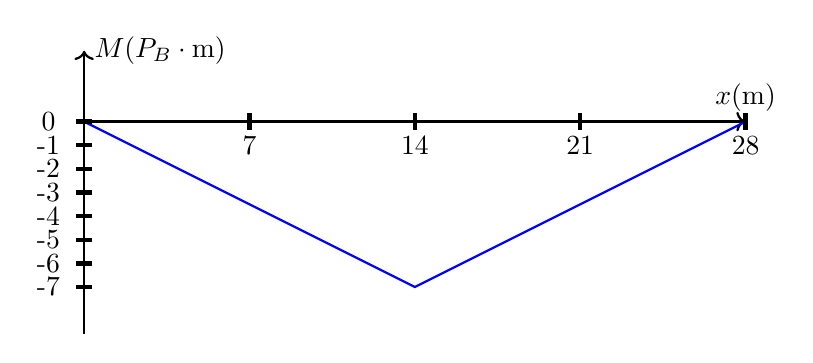
\begin{tikzpicture}[x=0.3cm,y=0.3cm]
      % Axis
      \draw[thick,->] (0,0) -- (28,0) node[above] {$x(\si{\meter})$};
      \draw[thick,->] (0,-9) -- (0,3) node[right] {$M(P_B \cdot \si{\meter})$};

      % Actual Plot
      \draw[thick, blue] (0,0) -- (14,-7) -- (28,0);

      % X axis
      \foreach \x in {7,14,21,28}
      {        
        \coordinate (A\x) at ($(0,0)+(\x,0)$) {};
        \draw[ultra thick] ($(A\x)+(0,3pt)$) -- ($(A\x)-(0,3pt)$);
        \node at ($(A\x)+(0ex,-2ex)$) {\x};
      }

      % Y Axis
      \foreach \y in {-7,...,0}
      {        
        \coordinate (B\y) at ($(0,0)+(0,\y)$) {};
        \draw[ultra thick] ($(B\y)+(3pt,0)$) -- ($(B\y)-(3pt,0)$);
        \node at ($(B\y)+(-3ex,0)$) {\y};
      }
  \end{tikzpicture}
\end{center}
Abusing symmetry once again, the displacement of $C$ relative to $B$ is:
\begin{equation}
  \delta_{CB}= 628.83 = \frac{1}{EI} \left(\frac{2}{3}(7000)\right)\left(\frac{1}{2}(14000^2)P_B\right) = 2.2866P_B
  \label{eq:}
\end{equation}
and solving for $P_B$ gives:
\begin{equation}
  P_B = 275\si{\kilo\newton}
  \label{eq:}
\end{equation}
\textbf{(c)} With $P_B=275\si{\kilo\newton}$, the forces the two supports exert is:
\begin{equation}
  A_y=C_y=\frac{1}{2}\left(200+200-275\right)=62.5\si{\kilo\newton}
  \label{eq:}
\end{equation}
such that the shear force diagram is:
\begin{center}
  \begin{tikzpicture}[x=0.3cm,y=0.03cm]
      % Axis
      \draw[thick,->] (0,0) -- (28,0) node[above] {$x(\si{\meter})$};
      \draw[thick,->] (0,-160) -- (0,160) node[right] {$V(\si{\kilo\newton})$};

      % Actual Plot
      \draw[thick, blue] (0,0) -- (0,62.5) -- (7,62.5) -- (7,-137.5) -- (14,-137.5) -- (14,137.5) -- (21,137.5) -- (21,-62.5) -- (28,-62.5) -- (28,0);

      % X axis
      \foreach \x in {7,14,21,28}
      {        
        \coordinate (A\x) at ($(0,0)+(\x,0)$) {};
        \draw[ultra thick] ($(A\x)+(0,3pt)$) -- ($(A\x)-(0,3pt)$);
        \node at ($(A\x)+(0ex,-2ex)$) {\x};
      }

      % Y Axis
      \foreach \y in {62.5,-137.5,137.5,-62.5,0}
      {        
        \draw[ultra thick] ($(0,\y)+(3pt,0)$) -- ($(0,\y)-(3pt,0)$);
        \node at ($(0,\y)+(-5ex,0)$) {\y};
      }

      % \draw[dotted] (7,62.5) -- (9,62.5) node[right] {$62.5$};
      % \draw[dotted] (7,-137.5) -- (9,62.5) node[right] {$62.5$};
      % \draw[dotted] (7,62.5) -- (9,62.5) node[right] {$62.5$};
      % \draw[dotted] (7,62.5) -- (9,62.5) node[right] {$62.5$};

  \end{tikzpicture}
\end{center}
and the shear force diagram as:
\begin{center}
  \begin{tikzpicture}[x=0.3cm,y=0.01cm]
      % Axis
      \draw[thick,->] (0,0) -- (28,0) node[above] {$x(\si{\meter})$};
      \draw[thick,->] (0,-550) -- (0,450) node[right] {$M(\si{\kilo\newton\meter})$};

      % Actual Plot
      \draw[thick, blue] (0,0) -- (7,437.5) -- (14,-525) -- (21,437.5) -- (28,0);

      % X axis
      \foreach \x in {7,14,21,28}
      {        
        \coordinate (A\x) at ($(0,0)+(\x,0)$) {};
        \draw[ultra thick] ($(A\x)+(0,3pt)$) -- ($(A\x)-(0,3pt)$);
        \node at ($(A\x)+(0ex,-2ex)$) {\x};
      }

      % Y Axis
      \foreach \y in {0,437.5,-525}
      {        
        \draw[ultra thick] ($(0,\y)+(3pt,0)$) -- ($(0,\y)-(3pt,0)$);
        \node at ($(0,\y)+(-5ex,0)$) {\y};
      }

      % \draw[dotted] (7,62.5) -- (9,62.5) node[right] {$62.5$};
      % \draw[dotted] (7,-137.5) -- (9,62.5) node[right] {$62.5$};
      % \draw[dotted] (7,62.5) -- (9,62.5) node[right] {$62.5$};
      % \draw[dotted] (7,62.5) -- (9,62.5) node[right] {$62.5$};

  \end{tikzpicture}
\end{center}
\newpage
\section{Problem Four}
The maximum shear force occurs at the ends and it has a magnitude of:
\begin{equation}
  V = \frac{1}{2}\left(5.5\si{\kilo\newton\per\meter}\cdot 3.5\si{\meter}\right) = 9.625\si{\kilo\newton}
  \label{eq:}
\end{equation}
The maximum shear stress occurs at the center of the beam, which has a moment of area equal to:
\begin{equation}
  Q = Ad = \left(90 \cdot \frac{180}{2}\right)\left(\frac{1}{2}180-\frac{1}{2}\frac{180}{2}\right) = 364500 \si{\milli\meter\cubed}
  \label{eq:allan fan club}
\end{equation}
The moment of inertia is equal to:
\begin{equation}
  I = \frac{1}{12}(90)(180^3) = 43.74 \times 10^6 \si{\milli\meter\tothe{4}}
  \label{eq:}
\end{equation}

such that the maximum shear stress is:
\begin{equation}
  \tau = \frac{VQ}{Ib} = \frac{(9625)(364500)}{(43.74 \times 10^6)(90)} = \boxed{0.891 \si{\mega\pascal}}
  \label{eq:}
\end{equation}
We can generalize equation \ref{eq:allan fan club} to:
\begin{equation}
  Q = Ad = \left(90 \cdot y\right)\left(\frac{180}{2}-\frac{y}{2}\right) = 45y\left(180-y\right)
  \label{eq:}
\end{equation}
and the shear stress distribution looks like this:
\begin{center}
  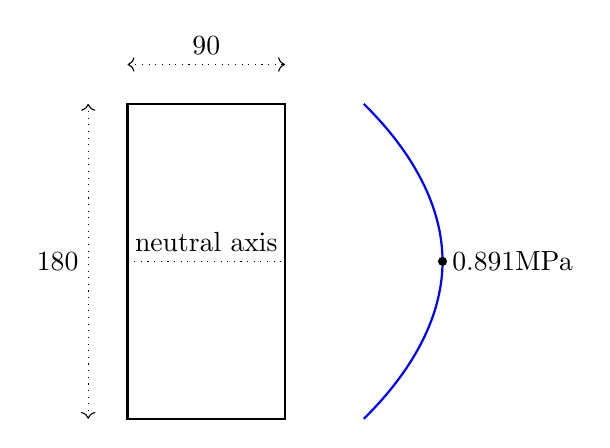
\begin{tikzpicture}[scale=1]
    \draw[rotate=-90,blue,thick] (-2,3) parabola bend (0,4) (2,3);
    \draw[thick] (0,-2) rectangle (2,2);

    \draw[dotted] (0,0) -- (2,0) node[midway,above] {$\text{neutral axis}$};
    \draw[dotted,<->] (-0.5,-2) -- (-0.5,2) node[midway,left] {$180$};
    \draw[dotted,<->] (0,2.5) -- (2,2.5) node[midway,above] {$90$};

    \draw[fill=black] (4,0) circle (0.05) node[right] {$0.891\si{\mega\pascal}$};
    % \path[thick,draw] (0,2) .. controls (2,2) and (2,-2) .. (0,-2);
  \end{tikzpicture}
\end{center}
\end{document}